\chapter{Thiết kế và hiện thực hệ thống}
\label{chap:implementation}\label{sec:impl}

\section{Yêu cầu hệ thống}\label{sec:yeucau}

Về chức năng, hệ thống phải đọc được bốn bộ dữ liệu, lọc ngoại lai nhân quả, chuẩn hoá và chia dữ liệu theo cell, với bộ
nhớ đệm để không phải đọc lại dữ liệu mỗi lần chạy. Mỗi thí nghiệm được định nghĩa thành một danh sách lượt huấn luyện,
chạy song song và chạy tiếp được sau khi dừng giữa chừng. Khối phân tích tính chỉ số theo cell, chạy kiểm định ghép cặp
và vẽ bảng, hình. Báo cáo này và bản thảo bài báo được sinh trực tiếp từ kết quả phân tích. Cuối cùng, hệ thống có một
công cụ dòng lệnh để ước lượng, dự báo và cập nhật SOH cho một cell từ tệp dữ liệu sạc của nó.

Về phi chức năng, có bốn yêu cầu. Bốn quy tắc chống rò rỉ ở \Cref{sec:protocol} phải được cài sẵn trong mã, không phụ
thuộc người chạy. Kết quả phải tái lập được: cùng phiên bản thư viện và cùng loại CPU thì chạy lại cho kết quả giống hệt.
Toàn bộ phải chạy được trên máy tính cá nhân, không cần GPU. Mỗi lượt chạy phải ghi đủ cấu hình, chỉ số và dự đoán vào
một tệp riêng để truy vết được.

\section{Kiến trúc hệ thống}\label{sec:kientruc}

Hệ thống được hiện thực bằng Python thành một đường ống năm bước: dữ liệu, tiền xử lý, thí nghiệm, phân tích và báo cáo
(Hình~\ref{fig:pipeline}). Toàn bộ đường ống chạy được từ dữ liệu tới báo cáo bằng một lệnh. Mỗi lượt huấn luyện là một
tệp kết quả độc lập, ghi đủ cấu hình, chỉ số, dự đoán trên tập xác thực và tập kiểm tra. Bộ lập lịch chạy song song nhiều
tiến trình một luồng và bỏ qua lượt đã có kết quả, nên chạy tiếp được sau khi dừng. Khối phân tích chỉ đọc các tệp kết
quả, không huấn luyện lại. Báo cáo này và bản thảo bài báo được sinh từ kết quả phân tích, nên mọi bảng đều khớp với dữ
liệu. Mọi lượt chạy trên CPU với một luồng và hạt giống cố định, nên chạy lại cho kết quả giống hệt
(Mục~\ref{sec:tailap}).

\begin{figure}[!htbp]\centering
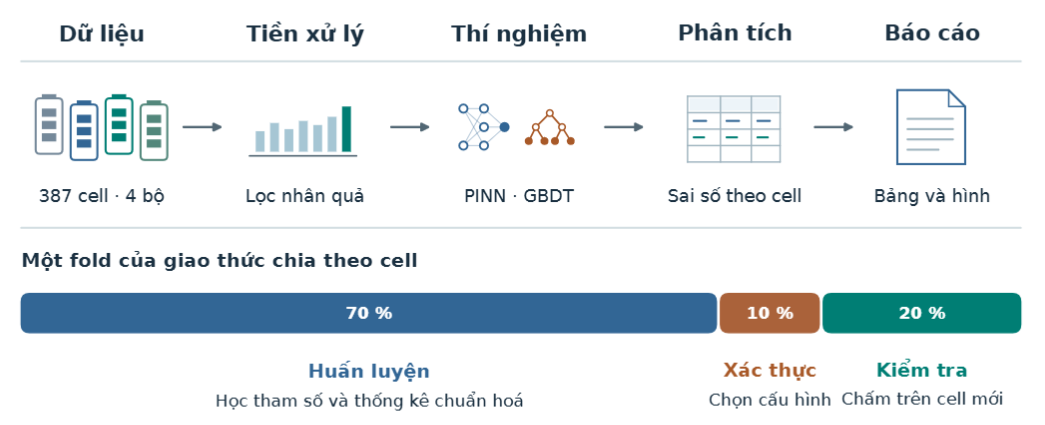
\includegraphics[width=\textwidth]{graphics/fig_quy_trinh.png}
\caption[Quy trình thực nghiệm và cách chia cell]{Quy trình thực nghiệm và cách chia cell: dữ liệu 387 cell của bốn bộ, tiền
xử lý với bộ lọc nhân quả, các thí nghiệm PINN và GBDT, phân tích sai số theo cell, rồi bảng và hình của báo cáo. Mỗi fold
dành 70\,\% số cell để huấn luyện (học tham số và thống kê chuẩn hoá), 10\,\% để xác thực (chọn cấu hình) và 20\,\% để
kiểm tra (chấm trên cell mới).}\label{fig:pipeline}
\end{figure}

\Cref{fig:modules} cho các khối mã nguồn và luồng dữ liệu giữa chúng. Thư viện lõi chứa mọi thứ cần để học và dự đoán:
đọc dữ liệu và chia theo cell, các mô hình ước lượng, các mô hình đối chứng, mô hình cập nhật và mô hình dự báo, cùng định
nghĩa thí nghiệm và bộ chạy song song. Kết quả mỗi lượt được ghi vào thư mục kết quả lượt chạy. Khối phân tích đọc thư mục
này, tính chỉ số theo cell và kiểm định, rồi ghi bảng và hình. Khối báo cáo đọc các bảng đó để sinh các đoạn văn có số,
các bảng \LaTeX{} và dựng PDF. Công cụ dòng lệnh dùng lại đúng các mô hình của thư viện lõi, còn khối so sánh chạy lại mã
gốc PINN4SOH trên cách chia của bài. Bảng~\ref{tab:exps} liệt kê các thí nghiệm có kết quả trong báo cáo.

\begin{figure}[!htbp]\centering
\begin{tikzpicture}[
  font=\footnotesize,
  box/.style={draw=black!55, rounded corners=2pt, fill=black!4, align=left, inner sep=4pt, text width=#1},
  box/.default=4.6cm,
  lib/.style={box=4.6cm, fill=blue!5, draw=blue!45!black},
  arr/.style={-{Stealth[length=2mm]}, draw=black!65, line width=0.6pt},
  node distance=3mm and 6mm]
\node[box=3.3cm] (data) {\textbf{Dữ liệu}\\ \texttt{PINN4SOH/data}: 16 đặc trưng sạc và dung lượng của 387 cell};
\node[lib, right=8mm of data, yshift=24mm] (d) {\texttt{data.py}: đọc, lọc ngoại lai nhân quả, chuẩn hoá, chia fold theo cell, đặc trưng lịch sử};
\node[lib, below=of d] (m) {\texttt{models.py}, \texttt{train.py}: PINN-semi, MLP, PINN hộp đen; huấn luyện, dừng sớm};
\node[lib, below=of m] (b) {\texttt{baselines.py}, \texttt{seqmodels.py}: Ridge, GPR, GBDT, CNN, LSTM, Transformer};
\node[lib, below=of b] (u) {\texttt{update.py}, \texttt{update\_hist.py}: GBDT-cập nhật, HiGBDT-$\Delta$, -R, -V};
\node[lib, below=of u] (f) {\texttt{forecast*.py}, \texttt{hipinn.py}: HiGBDT, PINN-dự báo, nhánh theo đời, HiPINN};
\node[lib, below=of f] (e) {\texttt{experiments.py}, \texttt{runner.py}: định nghĩa lượt chạy, chạy song song, chạy tiếp};
\begin{scope}[on background layer]
\node[draw=blue!45!black, dashed, rounded corners=3pt, inner sep=3pt, fit=(d)(e),
      label={[font=\footnotesize\bfseries, anchor=south]north:thư viện lõi \texttt{pinnsoh/}}] (core) {};
\end{scope}
\node[box=3.6cm, right=8mm of m] (runs) {\textbf{Kết quả lượt chạy}\\ \texttt{runs/}: một tệp JSON hoặc NPZ mỗi lượt (cấu hình, chỉ số, dự đoán)};
\node[box=3.6cm, below=5mm of runs] (an) {\textbf{Phân tích}\\ \texttt{analysis/}: MAE theo cell, kiểm định Wilcoxon--Holm, bảng CSV, hình};
\node[box=3.6cm, below=5mm of an] (rep) {\textbf{Báo cáo}\\ \texttt{report/build.py}: đoạn văn có số, bảng \LaTeX, PDF};
\node[box=3.6cm, below=5mm of rep] (tool) {\textbf{Công cụ dòng lệnh}\\ \texttt{tools/demo.py}: \texttt{train}, \texttt{predict}, \texttt{forecast}, \texttt{cap-nhat}};
\node[box=3.3cm, below=6mm of data] (run) {\textbf{Điều phối}\\ \texttt{run.py}: một lệnh cho mọi bước};
\node[box=3.3cm, below=4mm of run] (bench) {\textbf{So sánh}\\ \texttt{benchmark/}: mã gốc PINN4SOH trên cách chia của bài};
\draw[arr] (data.east) -- (core.west |- data.east);
\draw[arr] (core.east |- runs.west) -- (runs.west);
\draw[arr] (runs) -- (an);
\draw[arr] (an) -- (rep);
\draw[arr] (core.east |- tool.west) -- (tool.west);
\draw[arr] (run.east) -- (core.west |- run.east);
\draw[arr] (bench.east) -- (core.west |- bench.east);
\end{tikzpicture}
\caption[Các khối mã nguồn và luồng dữ liệu]{Các khối mã nguồn và luồng dữ liệu. Thư viện lõi chứa mọi mô hình và bộ
chạy thí nghiệm; mỗi lượt chạy ghi một tệp kết quả; khối phân tích chỉ đọc các tệp này; khối báo cáo sinh bảng và lời văn
có số từ kết quả phân tích; công cụ dòng lệnh dùng lại các mô hình của thư viện lõi.}\label{fig:modules}
\end{figure}

\begin{table}[!t]\centering\small
\caption[Các thí nghiệm có kết quả trong báo cáo]{Các thí nghiệm có kết quả trong báo cáo và số lượt huấn luyện (mỗi lượt là một mô hình trên một fold, hoặc một lần chạy trên một nhóm; lượt trùng cấu hình chỉ tính một lần).}\label{tab:exps}
\begin{tabularx}{\textwidth}{>{\raggedright\arraybackslash}X r}\toprule
Thí nghiệm & Lượt \\\midrule
Kiểm định chéo chính: MLP, PINN-semi ở 4 mức nhãn; PINN-sup và hai biến thể lược bỏ thành phần ở 30\,\% & 1.100 \\
Kiểm toán rò rỉ: 4 cách chia và chuẩn hoá sai, MLP 70\,\% nhãn & 160 \\
Ridge, GPR, GBDT ở 4 mức nhãn & 1.200 \\
PINN-sup ở 10 và 50\,\%; PINN hộp đen ở 4 mức nhãn & 600 \\
PINN-lai: 9 hướng cải tiến chọn trên tập xác thực; 3 PINN-semi, GBDT, 3 lần lặp, 4 mức nhãn & 1.680 \\
CNN, LSTM, Transformer: chọn độ dài cửa sổ trên tập xác thực; 3 lần lặp, 4 mức nhãn & 840 \\
Đầu vào có lịch sử của cell: chọn dạng trên tập xác thực; PINN-semi, MLP, GBDT & 1.190 \\
Ngân sách đo: đo thưa mọi cell huấn luyện theo 4 lịch đo & 1.560 \\
GBDT-cập nhật: cập nhật SOH từ lần đo gần nhất & 240 \\
Dự báo SOH, dung lượng, RUL: HiGBDT, HiPINN, các nhánh và mô hình đối chứng, 2 ngân sách nhãn, 3 lần lặp & 120 \\
HiGBDT cho bài toán cập nhật: GBDT-cập nhật, HiGBDT-$\Delta$, -R, -V trên 4 lịch đo & 60 \\
PINN-lai, GBDT và PINN-semi trên đúng 39 nhóm của PINN4SOH, 2 cách tiền xử lý, 3 hạt giống & 1.002 \\
Mã gốc PINN4SOH trên 39 nhóm đánh giá của bài, 10 lần mỗi nhóm & 390 \\
Phân tích đặc trưng: 120 fold $\times$ 9--10 lần huấn luyện GBDT với các tập đầu vào khác nhau & 1.110 \\
Độ nhạy của bộ lọc ngoại lai: GBDT với 7 cách đặt khác của bộ lọc, 4 bộ, 30\,\% nhãn & 420 \\
\midrule
Tổng & 11.672 \\
\bottomrule\end{tabularx}\end{table}


\section{Hiện thực}\label{sec:hienthuc}

Hệ thống viết bằng Python 3.11 với PyTorch 2.14 cho mạng nơ-ron, scikit-learn 1.9 cho Ridge, GPR và GBDT, cùng NumPy,
pandas, SciPy (kiểm định) và Matplotlib (hình). Báo cáo dựng bằng \LaTeX. Lệnh \texttt{python run.py} gọi mọi bước: tải dữ
liệu, chạy một hoặc mọi thí nghiệm, phân tích, dựng báo cáo và kiểm tra tái lập. Để chạy hơn mười nghìn lượt huấn luyện
trên CPU mà không đổi kết quả, hệ thống dùng năm kỹ thuật. Dữ liệu đã lọc được lưu vào bộ nhớ đệm, nên thời gian nạp bốn
bộ dữ liệu giảm từ 10,8\,s còn 0,02\,s. Tensor được dựng một lần cho cả lượt chạy. Việc dừng sớm chỉ tính MAE trên tập xác
thực. Các lượt dài được chạy trước và mỗi tiến trình dùng một luồng. Kết quả được ghi ra một tệp tạm rồi mới đổi tên thành
tệp chính thức, nên dừng giữa chừng không để lại tệp dở. Hình và PDF không ghi thời điểm tạo, nên dựng lại từ cùng dữ liệu
cho tệp giống hệt.

\section{Công cụ dự báo cho một cell}\label{sec:congcu}

Công cụ dòng lệnh của đồ án gói PINN-semi, HiPINN và HiGBDT-V để dùng cho một cell bất kỳ, chỉ cần tệp đặc trưng sạc của cell đó. Lệnh thứ nhất học PINN-semi ở 30\,\% nhãn cho một bộ dữ liệu, lệnh thứ hai ước lượng SOH ở từng chu kỳ, lệnh thứ ba dự báo SOH, dung lượng và RUL từ một chu kỳ bất kỳ bằng HiPINN (\Cref{sec:e33pp}). Lần đầu dự báo cho một bộ, HiPINN được học trên các cell có nhãn của cùng fold với PINN-semi của công cụ, chọn cấu hình từng nhánh trên cell validation rồi lưu lại; cell được dự báo không tham gia khi học. Lịch sử SOH tới gốc là dung lượng đo của chính cell; cell chưa được đo dung lượng thì công cụ chỉ ước lượng SOH hiện tại (lệnh thứ hai), không dự báo. Lệnh thứ tư cập nhật SOH khi cell được đo dung lượng ở vài chu kỳ: ở mỗi chu kỳ không đo, HiGBDT-V (\Cref{sec:anchor}) ước lượng SOH từ lần đo gần nhất trước nó và đặc trưng sạc. Với cell 2C\_battery-8 của XJTU đo 11 lần trên 385 chu kỳ theo lịch mỗi $0{,}1L$, MAE ở các chu kỳ không đo là 2{,}1 ($\times10^{-3}$), so với 8{,}7 khi giữ nguyên lần đo gần nhất.

Lệnh thứ năm áp dụng HiPINN cho cả bốn bộ: với mỗi bộ, lấy cell test có số chu kỳ ở trung vị và dự báo từ 40\,\% số chu kỳ của nó (\Cref{fig:demo4}). MAE trên phần đời còn lại là 23{,}3 ở XJTU (cell 2C\_battery-1), 6{,}9 ở TJU (cell CY25-025\_1-\#4), 10{,}8 ở MIT (cell 2017-05-12\_battery-43) và 3{,}8 ở HUST (cell 7-1) ($\times10^{-3}$); ở TJU và HUST, HiPINN không kém nhánh tốt nhất của chính cell đó; ở XJTU, nhánh tốt nhất là HiGBDT (16{,}9); ở MIT, nhánh tốt nhất là nhánh theo đời (9{,}6). Mô hình của công cụ học trên 30\,\% cell có nhãn, ít hơn mức mọi cell train ở \Cref{sec:e33res}, và mỗi bộ chỉ có một cell, nên đây là minh hoạ chứ không phải số đánh giá.

\begin{figure}[!htbp]\centering
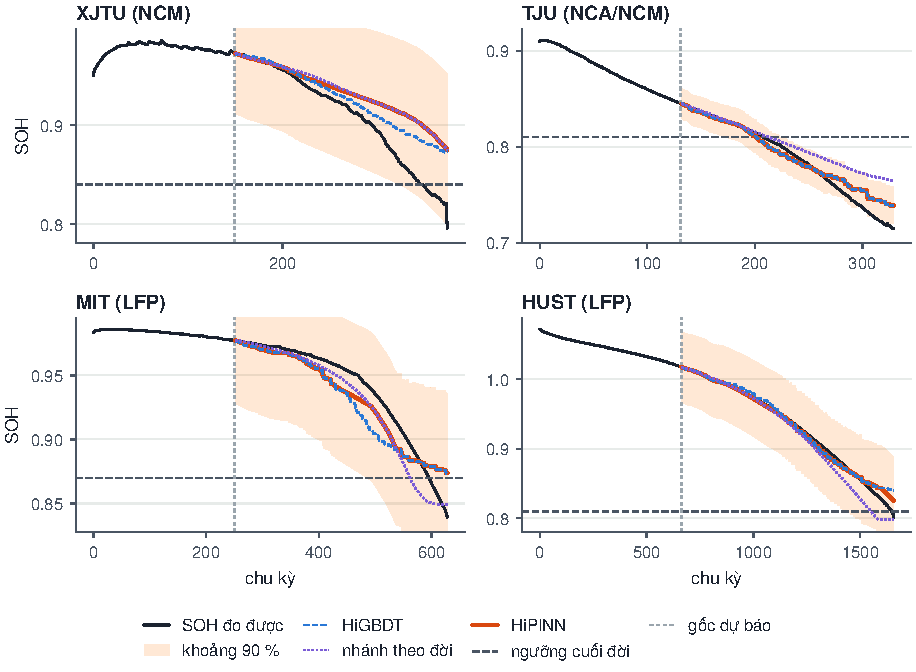
\includegraphics[width=\textwidth]{graphics/fig_demo_hipinn.pdf}
\caption[HiPINN cho một cell test của mỗi bộ dữ liệu]{HiPINN áp dụng cho bốn bộ dữ liệu qua công cụ dòng lệnh: với mỗi bộ, cell test có số chu kỳ ở trung vị, dự báo từ 40\,\% số chu kỳ của cell, lịch sử là dung lượng đo; mô hình học trên 30\,\% cell có nhãn của fold dùng cho công cụ. PINN-dự báo, nhánh thứ ba của HiPINN, không vẽ để hình dễ đọc.}\label{fig:demo4}
\end{figure}


Bảng~\ref{tab:cli} cho cú pháp các lệnh của công cụ. Tệp đầu vào là một tệp CSV với mỗi hàng là một chu kỳ, gồm 16 cột
đặc trưng sạc theo đúng tên trong bản dữ liệu của PINN4SOH và, nếu có, một cột \texttt{capacity} chứa dung lượng đo (Ah).
Mỗi lệnh ghi kết quả vào thư mục \texttt{demo/} dưới dạng một tệp CSV và một hình.

\begin{table}[!htbp]\centering\small
\caption[Cú pháp các lệnh của công cụ dòng lệnh]{Cú pháp các lệnh của công cụ dòng lệnh (\texttt{python tools/demo.py}
\textit{lệnh} \textit{tham số}). Tham số trong ngoặc vuông là không bắt buộc.}\label{tab:cli}
\begin{tabularx}{\textwidth}{>{\raggedright}p{6.4cm}>{\raggedright\arraybackslash}X}
\toprule
Lệnh và tham số & Chức năng \\
\midrule
\texttt{train --dataset XJTU} & học PINN-semi ở 30\,\% nhãn trên một fold của bộ dữ liệu, lưu \texttt{demo/XJTU.pt} \\
\texttt{predict --model demo/XJTU.pt --csv} \textit{tệp} \texttt{[--nominal} \textit{Ah}\texttt{] [--temp} \textit{°C}\texttt{]
[--an-nhan]} & ước lượng SOH ở từng chu kỳ; \texttt{--an-nhan} bỏ cột dung lượng để giả lập cell chưa đo \\
\texttt{forecast --model demo/XJTU.pt --csv} \textit{tệp} \texttt{[--den-chu-ky} \textit{k}\texttt{]} & dự báo SOH, dung lượng
và RUL bằng HiPINN từ chu kỳ gốc $k$ (mặc định chu kỳ cuối của tệp); cần dung lượng đo tới $k$ \\
\texttt{cap-nhat --model demo/XJTU.pt --csv} \textit{tệp} \texttt{[--lich q20|q10|q05]} \texttt{[--do-chu-ky "1,60,120"]} &
cập nhật SOH ở các chu kỳ không đo từ lần đo gần nhất bằng GBDT-cập nhật; lịch đo giả lập hoặc danh sách chu kỳ có đo \\
\texttt{tat-ca} & áp dụng HiPINN cho một cell kiểm tra của mỗi bộ, hình $2 \times 2$ \\
\bottomrule
\end{tabularx}
\end{table}

\section{Chi phí tính toán khi triển khai}\label{sec:chiphi}

BMS thường chạy trên vi điều khiển hoặc một máy tính nhúng có bộ nhớ và năng lực tính toán hạn chế, nên chi phí suy luận là một tiêu chí khi triển khai. \Cref{tab:cost} đo chi phí của hai mô hình cuối trên CPU một luồng. Mỗi mạng nghiệm của PINN-lai có 27.137 tham số. Khi suy luận chỉ cần mạng nghiệm, còn mạng tốc độ chỉ dùng lúc học. GBDT của PINN-lai có 100--1000 cây tuỳ bộ. Toàn bộ PINN-lai chiếm 705\,KB--3{,}7\,MB và cần 1{,}10--7{,}32\,ms cho mỗi chu kỳ mới, chủ yếu cho lượt dự đoán của GBDT (0{,}72--6{,}34\,ms), sau đó là ba lượt truyền thẳng (0{,}13--0{,}20\,ms). Bộ lọc xu thế chỉ cần nhớ 10 ước lượng gần nhất của cell. Với một lần đo mỗi chu kỳ sạc, chi phí này nhỏ so với thời gian một lần sạc. HiPINN nặng hơn: 4{,}5--10{,}3\,MB, lớn nhất ở HUST, trong đó nhánh theo đời (GBDT đời còn lại và khuôn quỹ đạo của các cell huấn luyện) chiếm 71--93\,\%. Một lần dự báo cho mọi tầm tới $3L$ mất 18--29\,ms. Dự báo không cần chạy ở mọi chu kỳ, nên HiPINN phù hợp với một máy chủ hay một bộ điều khiển có bộ nhớ từ 11\,MB trở lên, còn PINN-lai đủ nhẹ để chạy sau mỗi lần sạc trên một máy tính nhúng. Các số đo trên một lõi CPU của máy chạy thí nghiệm, không phải trên phần cứng của BMS. Trên vi điều khiển, độ trễ sẽ lớn hơn và cần đo lại.

\begin{table}[!htbp]\centering\small
\caption[Chi phí tính toán của PINN-lai và HiPINN]{Chi phí tính toán trên CPU một luồng của mô hình trong công cụ dòng lệnh (học ở 30\,\% nhãn trên một fold của mỗi bộ). Tham số mạng nghiệm tính cho một trong ba mạng của PINN-lai; dung lượng là kích thước khi lưu; độ trễ là trung vị của nhiều lần gọi. PINN-lai: một chu kỳ mới (ba mạng nghiệm, GBDT cho một hàng, bộ lọc xu thế). HiPINN: một lần dự báo từ một gốc cho mọi tầm tới $3L$, gồm cả tính đặc trưng lịch sử của cell.}\label{tab:cost}
\begin{tabular}{lrrrrrr}\toprule
 & \multicolumn{4}{c}{PINN-lai} & \multicolumn{2}{c}{HiPINN} \\\cmidrule(lr){2-5}\cmidrule(lr){6-7}
Bộ & \begin{tabular}[b]{@{}r@{}}tham số\\mạng nghiệm\end{tabular} & \begin{tabular}[b]{@{}r@{}}số cây\\GBDT\end{tabular} & \begin{tabular}[b]{@{}r@{}}dung\\lượng\end{tabular} & \begin{tabular}[b]{@{}r@{}}độ trễ\\(ms/chu kỳ)\end{tabular} & \begin{tabular}[b]{@{}r@{}}dung\\lượng\end{tabular} & \begin{tabular}[b]{@{}r@{}}độ trễ\\(ms/dự báo)\end{tabular} \\\midrule
XJTU & 27.137 & 850 & 3{,}2\,MB & 5{,}90 & 4{,}5\,MB & 18 \\
TJU & 27.137 & 1000 & 3{,}7\,MB & 7{,}32 & 6{,}3\,MB & 19 \\
MIT & 27.137 & 850 & 3{,}2\,MB & 5{,}72 & 8{,}5\,MB & 29 \\
HUST & 27.137 & 100 & 705\,KB & 1{,}10 & 10{,}3\,MB & 18 \\
\bottomrule\end{tabular}\end{table}

